\begin{enumerate}[label=\thechapter.\arabic*,ref=\thechapter.\theenumi]
\item In the complex $z$-domain, the value of integral $\oint_{C}\frac{z^3-9}{3z-i}\;dz$ is   \\
\begin{enumerate}[label=(\alph*)]
    \item $\frac{2\pi}{81}-6i\pi$ 
    \item $\frac{2\pi}{81}+6i\pi$ 
    \item $-\frac{2\pi}{81}+6i\pi$ 
    \item $-\frac{2\pi}{81}-6i\pi$ 
\end{enumerate} \hfill(GATE 2022 BM)    \\
\solution
% \iffalse
\let\negmedspace\undefined
\let\negthickspace\undefined
\documentclass[journal,12pt,twocolumn]{IEEEtran}
\usepackage{cite}
\usepackage{amsmath,amssymb,amsfonts,amsthm}
\usepackage{algorithmic}
\usepackage{graphicx}
\usepackage{textcomp}
\usepackage{xcolor}
\usepackage{txfonts}
\usepackage{listings}
\usepackage{enumitem}
\usepackage{mathtools}
\usepackage{gensymb}
\usepackage{comment}
\usepackage[breaklinks=true]{hyperref}
\usepackage{tkz-euclide} 
\usepackage{listings}
\usepackage{gvv}                                        
\def\inputGnumericTable{}                                 
\usepackage[latin1]{inputenc}                                
\usepackage{color}                                            
\usepackage{array}                                            
\usepackage{longtable}                                       
\usepackage{calc}                                             
\usepackage{multirow}                                         
\usepackage{hhline}                                           
\usepackage{ifthen}                                           
\usepackage{lscape}

\newtheorem{theorem}{Theorem}[section]
\newtheorem{problem}{Problem}
\newtheorem{proposition}{Proposition}[section]
\newtheorem{lemma}{Lemma}[section]
\newtheorem{corollary}[theorem]{Corollary}
\newtheorem{example}{Example}[section]
\newtheorem{definition}[problem]{Definition}
\newcommand{\BEQA}{\begin{eqnarray}}
\newcommand{\EEQA}{\end{eqnarray}}
\newcommand{\define}{\stackrel{\triangle}{=}}
\theoremstyle{remark}
\newtheorem{rem}{Remark}
\begin{document}
\parindent 0px
\bibliographystyle{IEEEtran}
\title{GATE: BM - 36.2022}
\author{EE22BTECH11219 - Rada Sai Sujan$^{}$% <-this % stops a space
}
\maketitle
\newpage
\bigskip
\section*{Question}
In the complex $z$-domain, the value of integral $\oint_{C}\frac{z^3-9}{3z-i}\;dz$ is   \\
\begin{enumerate}[label=(\alph*)]
    \item $\frac{2\pi}{81}-6i\pi$ 
    \item $\frac{2\pi}{81}+6i\pi$ 
    \item $-\frac{2\pi}{81}+6i\pi$ 
    \item $-\frac{2\pi}{81}-6i\pi$ 
\end{enumerate} \hfill(GATE 2022 BM)    \\
\solution

Simplyfying the Contour Integral to the standard form we get,
\begin{align}
    \oint_{C}\frac{z^3-9}{3z-i}\;dz &= \frac{1}{3}\oint_{C}\frac{z^3-9}{z-\frac{i}{3}}\;dz
\end{align}
From Cauchy's residue theorem,
\begin{align}
    \oint_{C}f(z)\;dz &= 2\pi i\sum R_j \label{equation:bm.2022.36Q.2}
\end{align}
We can observe a non-repeated pole at $z=\frac{i}{3}$ and thus $a=\frac{i}{3}$,
\begin{align}
    R &= \lim\limits_{z\to a}\brak{z-a}f\brak{z}    \\
    \implies R &= \frac{1}{3}\lim\limits_{z\to \frac{i}{3}}\brak{z-\frac{i}{3}}\frac{z^3-9}{z-\frac{i}{3}}  \\
    &= \frac{-i}{81}-3  \label{equation:bm.2022.36Q.5}
\end{align}
Therefore, from \eqref{equation:bm.2022.36Q.2} and \eqref{equation:bm.2022.36Q.5}
\begin{align}
    \oint_{C}\frac{z^3-9}{3z-i}\;dz &= \frac{2\pi}{81}-6i\pi
\end{align}
\end{document}

\newpage
\item Consider the function
\begin{align*}
f\brak{z} = \frac{1}{\brak{z+1}\brak{z+2}\brak{z+3}}
\end{align*}
The residue of $f\brak{z}$ at $z=-1$, is \rule{1cm}{0.15mm}
\hfill(GATE 2022 IN) \\
\solution
\iffalse
\let\negmedspace\undefined
\let\negthickspace\undefined
\documentclass[journal,12pt,twocolumn]{IEEEtran}
\usepackage{cite}
\usepackage{amsmath,amssymb,amsfonts,amsthm}
\usepackage{algorithmic}
\usepackage{graphicx}
\usepackage{textcomp}
\usepackage{xcolor}
\usepackage{txfonts}
\usepackage{listings}
\usepackage{enumitem}
\usepackage{mathtools}
\usepackage{gensymb}
\usepackage{comment}
\usepackage[breaklinks=true]{hyperref}
\usepackage{tkz-euclide}
\usepackage{listings}
\usepackage{gvv}
\def\inputGnumericTable{}
\usepackage[latin1]{inputenc}
\usepackage{color}
\usepackage{array}
\usepackage{longtable}
\usepackage{calc}
\usepackage{multirow}
\usepackage{hhline}
\usepackage{ifthen}
\usepackage{lscape}

\newtheorem{theorem}{Theorem}[section]
\newtheorem{problem}{Problem}
\newtheorem{proposition}{Proposition}[section]
\newtheorem{lemma}{Lemma}[section]
\newtheorem{corollary}[theorem]{Corollary}
\newtheorem{example}{Example}[section]
\newtheorem{definition}[problem]{Definition}
\newcommand{\BEQA}{\begin{eqnarray}}
\newcommand{\EEQA}{\end{eqnarray}}
\newcommand{\define}{\stackrel{\triangle}{=}}
\theoremstyle{remark}
\newtheorem{rem}{Remark}
\begin{document}

\bibliographystyle{IEEEtran}
\vspace{3cm}

\title{GATE 2022 IN 61}
\author{EE23BTECH11007 - Aneesh Kadiyala$^{*}$% <-this % stops a space
}
\maketitle
\newpage
\bigskip

\renewcommand{\thefigure}{\theenumi}
\renewcommand{\thetable}{\theenumi}

\vspace{3cm}
\textbf{Question:} Consider the function
\begin{align*}
f\brak{z} = \frac{1}{\brak{z+1}\brak{z+2}\brak{z+3}}
\end{align*}
The residue of $f\brak{z}$ at $z=-1$, is \rule{1cm}{0.15mm}

\hfill(GATE 2022 IN 61)
\\
\solution
\\
\fi
Residue of a function $f\brak{z}$ at a simple pole $c$ is
\begin{align}
\text{Res}\brak{f, c} &= \lim_{z \to c}\brak{z - c}f\brak{z} \\
\implies \text{Res}\brak{f,-1} &= \lim_{z \to -1}\frac{z + 1}{\brak{z+1}\brak{z+2}\brak{z+3}} \\
&= \frac{1}{2}
\end{align}
$\therefore$ residue of $f\brak{z}$ at $z = -1$ is $\frac{1}{2}$.
\newpage

\item The value of the integral 
\begin{align*}
    \int_C \frac{z^{100}}{z^{101}+1}\, dz
\end{align*}
where $C$ is the circle of radius 2 centred at the origin taken in the anti-clockwise direction is\\
\begin{enumerate}[label=(\Alph*)]
    \item $-2 \pi i$
    \item $2\pi$
    \item $0$
    \item $2\pi i $
\end{enumerate}
\hfill(GATE 2022 MA)\\
\solution\\
\iffalse
\documentclass[journal,12pt,twocolumn]{IEEEtran}
\usepackage{amsmath,amssymb,amsfonts,amsthm}
\usepackage{txfonts}
\usepackage{tkz-euclide}
\usepackage[margin=0.25in]{geometry}
\usepackage{pgfplots}
\usepackage{listings}
\usepackage{gvv}
\usepackage[latin1]{inputenc}
\usepackage{adjustbox}
\usepackage{array}
\usepackage{tabularx}
\usepackage{enumitem}
\usepackage{pgf}
\usepackage{lmodern}
\usepackage{circuitikz}
\usepackage{tikz}
\usepackage{graphicx}
\pgfplotsset{width=10cm,compat=1.18}

\begin{document}
\bibliographystyle{IEEEtran}

\vspace{3cm}

\title{}
\author{EE23BTECH11054 -  Sai Krishna Shanigarapu$^{*}$
}
\maketitle
\newpage
\bigskip

\section*{Gate MA 2022}
14. \hspace{2pt} The value of the integral 
\begin{align*}
    \int_C \frac{z^{100}}{z^{101}+1}\, dz
\end{align*}
where $C$ is the circle of radius 2 centred at the origin taken in the anti-clockwise direction is\\
\begin{enumerate}[label=(\Alph*)]
    \item $-2 \pi i$
    \item $2\pi$
    \item $0$
    \item $2\pi i $
\end{enumerate}
\hfill(GATE 2022 MA)\\
\solution\\
\fi
Using \ref{Cauchy} and \ref{Residue}
Solving the integral,
\begin{align}
f\brak{z} &= \int_C \frac{z^{100}}{z^{101}+1}\, dz
\end{align}

\begin{figure}[ht]
    \centering
    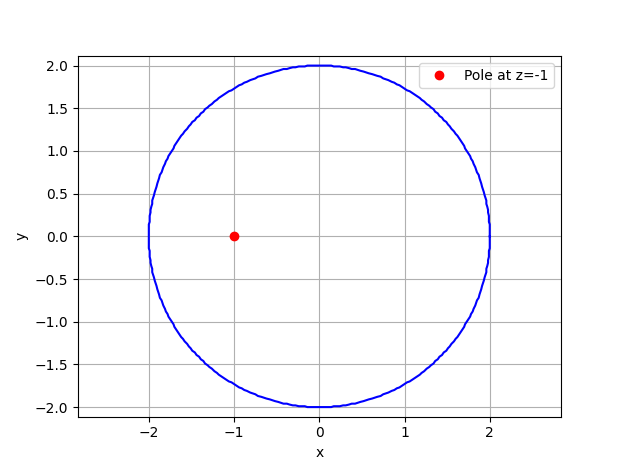
\includegraphics[width=\columnwidth]{2022/MA/14/figs/Figure_1.png}
    \caption{plot of $C$ with it's pole}
    \label{fig:fig1_gate_ma_2022_14_054}
\end{figure}
Since the pole $z=-1$ is inside the circle, Using eq (\ref{eq:eq2_gate_ma_2022_14_054})
\begin{align}
    Res\, f\brak{-1} &= \lim_{z\to -1}\brak{\frac{z^{100}}{z^{101}+1}}\brak{z^{101} + 1}\\
    &= 1 \label{eq:eq3_gate_ma_2022_14_054}
\end{align}

From eq (\ref{eq:eq1_gate_ma_2022_14_054}), and eq (\ref{eq:eq3_gate_ma_2022_14_054})
\begin{align}
    \int f\brak{z}\, dz &= 2\pi i \brak{1}\\
    \implies \int_C \frac{z^{100}}{z^{101}+1}\, dz &= 2 \pi i
\end{align}

$\therefore$ option (D) is correct.


%\end{document}

\end{enumerate}
